\section{Independent legal and scientific references}
\label{sec:natural-domains}
We froze a model-blind external-domain check using 144 document--hypothesis pairs from 91 ContractNLI test contracts \citep{contractnli} and 120 claim--cited-abstract pairs from SciFact's annotated development set \citep{scifact}. The legal sample has 48 cases per entailment, contradiction and not-mentioned label; the science sample has 60 support and 60 contradiction pairs. Both are intentionally balanced for paired sensitivity, not representative of natural label prevalence. Every pair receives original, byte-identical repeat and reversed-candidate requests; references and semantic candidate meanings remain unchanged. All 792 unique requests passed a complete-input audit for each of four local adapters. The hosted HTTP payloads were complete, although server-side tokenization is unobservable. Intervals below resample by contract or claim, respectively, and are pointwise unless stated otherwise.

Figure~\ref{fig:natural-main} partitions each domain's cases by correctness under both renderings. In law, the code-likelihood LLM adapters change 66/144 Llama and 64/144 Qwen semantic labels. Their reference agreement rises from 44 to 59 and from 65 to 83 out of 144, respectively, but only 33 and 51 cases are correct \emph{under both} renderings. Those net gains hide 26 corrections and 11 regressions for Llama, and 32 corrections and 14 regressions for Qwen. Pointwise contract-cluster intervals for the paired gains are $[+2.8,+18.3]$ and $[+4.2,+20.7]$ percentage points. These are not improvements in legal reasoning: ordinary reversal changes answer-code assignment in the adapters, and Section~\ref{sec:domain-codebook} isolates that confound.

On scientific evidence, the direction need not match. Qwen loses eight correct decisions ($92/120\to84/120$, $-6.7$ points, claim-cluster interval $[-12.5,-0.8]$), while Jev is reference-correct on the same 112/120 pairs under both orders. Jev's legal original/reversal agreement is 138/144, compared with 142/144 on a literal repeat. These selected-pair observations are not a ranking of legal or scientific competence across native interfaces. The SciFact diagnostic contains only positive evidence relations attached to a cited abstract: it neither tests retrieval nor samples no-information decisions. A separately frozen three-class extension including no-information is kept distinct from this denominator.

\begin{figure}[t]
\centering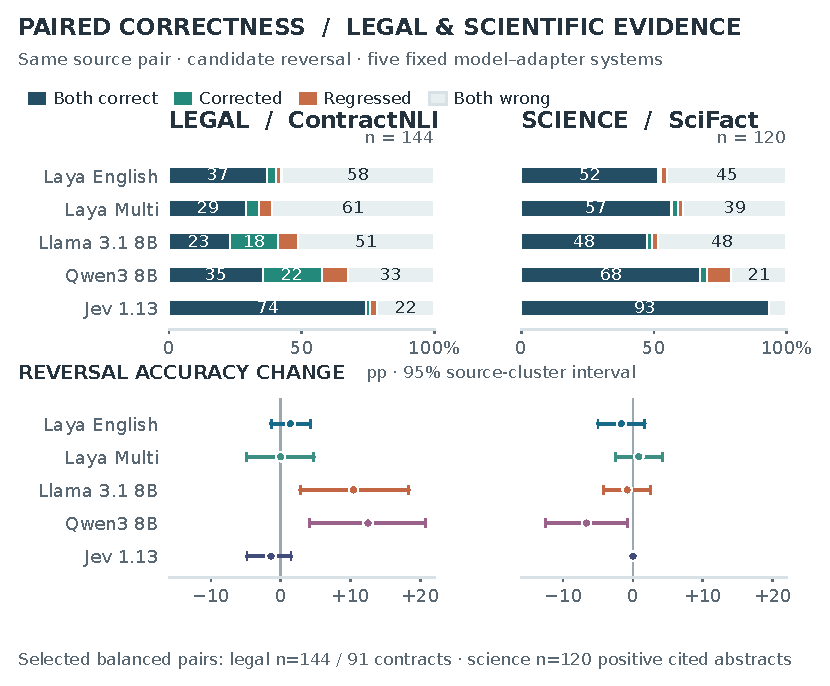
\includegraphics[width=.99\linewidth]{figures/fig_domain_expansion_main.pdf}
\caption{Paired correctness under ordinary candidate reversal on selected, class-balanced ContractNLI and SciFact source pairs. Each bar partitions the same pairs into both-correct, corrected, regressed and both-wrong cases; lower panels show reversal-minus-base accuracy with pointwise 95\% source-cluster bootstrap intervals. The LLM intervention jointly changes display and code assignment; the science sample excludes retrieval/no-information.}
\label{fig:natural-main}
\label{fig:natural-domains}
\end{figure}
